\documentclass[a4paper, 12pt, margins=2.5cm]{homework}
\usepackage{tikz}

\usepackage{graphicx}
\usepackage{dsfont}
\usepackage{microtype}
\usepackage{mathrsfs}
\usepackage[ngerman]{babel}
\usepackage{csquotes}
\usepackage[T1]{fontenc}
\usepackage{lmodern}
\usepackage{wasysym}

\setlength{\parindent}{0pt}

\newcommand{\R}{\mathbb{R}}
\newcommand{\N}{\mathbb{N}}
\newcommand{\Z}{\mathbb{Z}}
\newcommand{\Q}{\mathbb{Q}}
\newcommand{\C}{\mathbb{C}}

\name{Tobias Eidelpes}
\course{Objektorientierte Modellierung}
\term{2016SS}
\hwnum{5}
\hwtype{Übungsblatt}
\problemtitle{Aufgabe}
\solutiontitle{Lösung}

\begin{document}
  

  \problemnumber{1}
  \begin{problem}
    
  \end{problem}
  \begin{solution}\hfill
    \begin{enumerate}[label=\alph*)]\itemsep0pt
      \item Eine Aktivität ist ein gerichteter Graph. In diesem Graphen sind die
            Knoten die Aktionen. Aktionen sind im Gegensatz zu Aktivitäten atomar.
            Aktivitäten bestehen selbst aus mehreren Teilen (Aktionen), wobei 
            Aktionen nicht mehr unterteilt werden können. Außerdem kann ich bei
            Aktivitäten Eingabe- und Ausgabeparameter festlegen.

      \item \hfill
        \begin{center}
          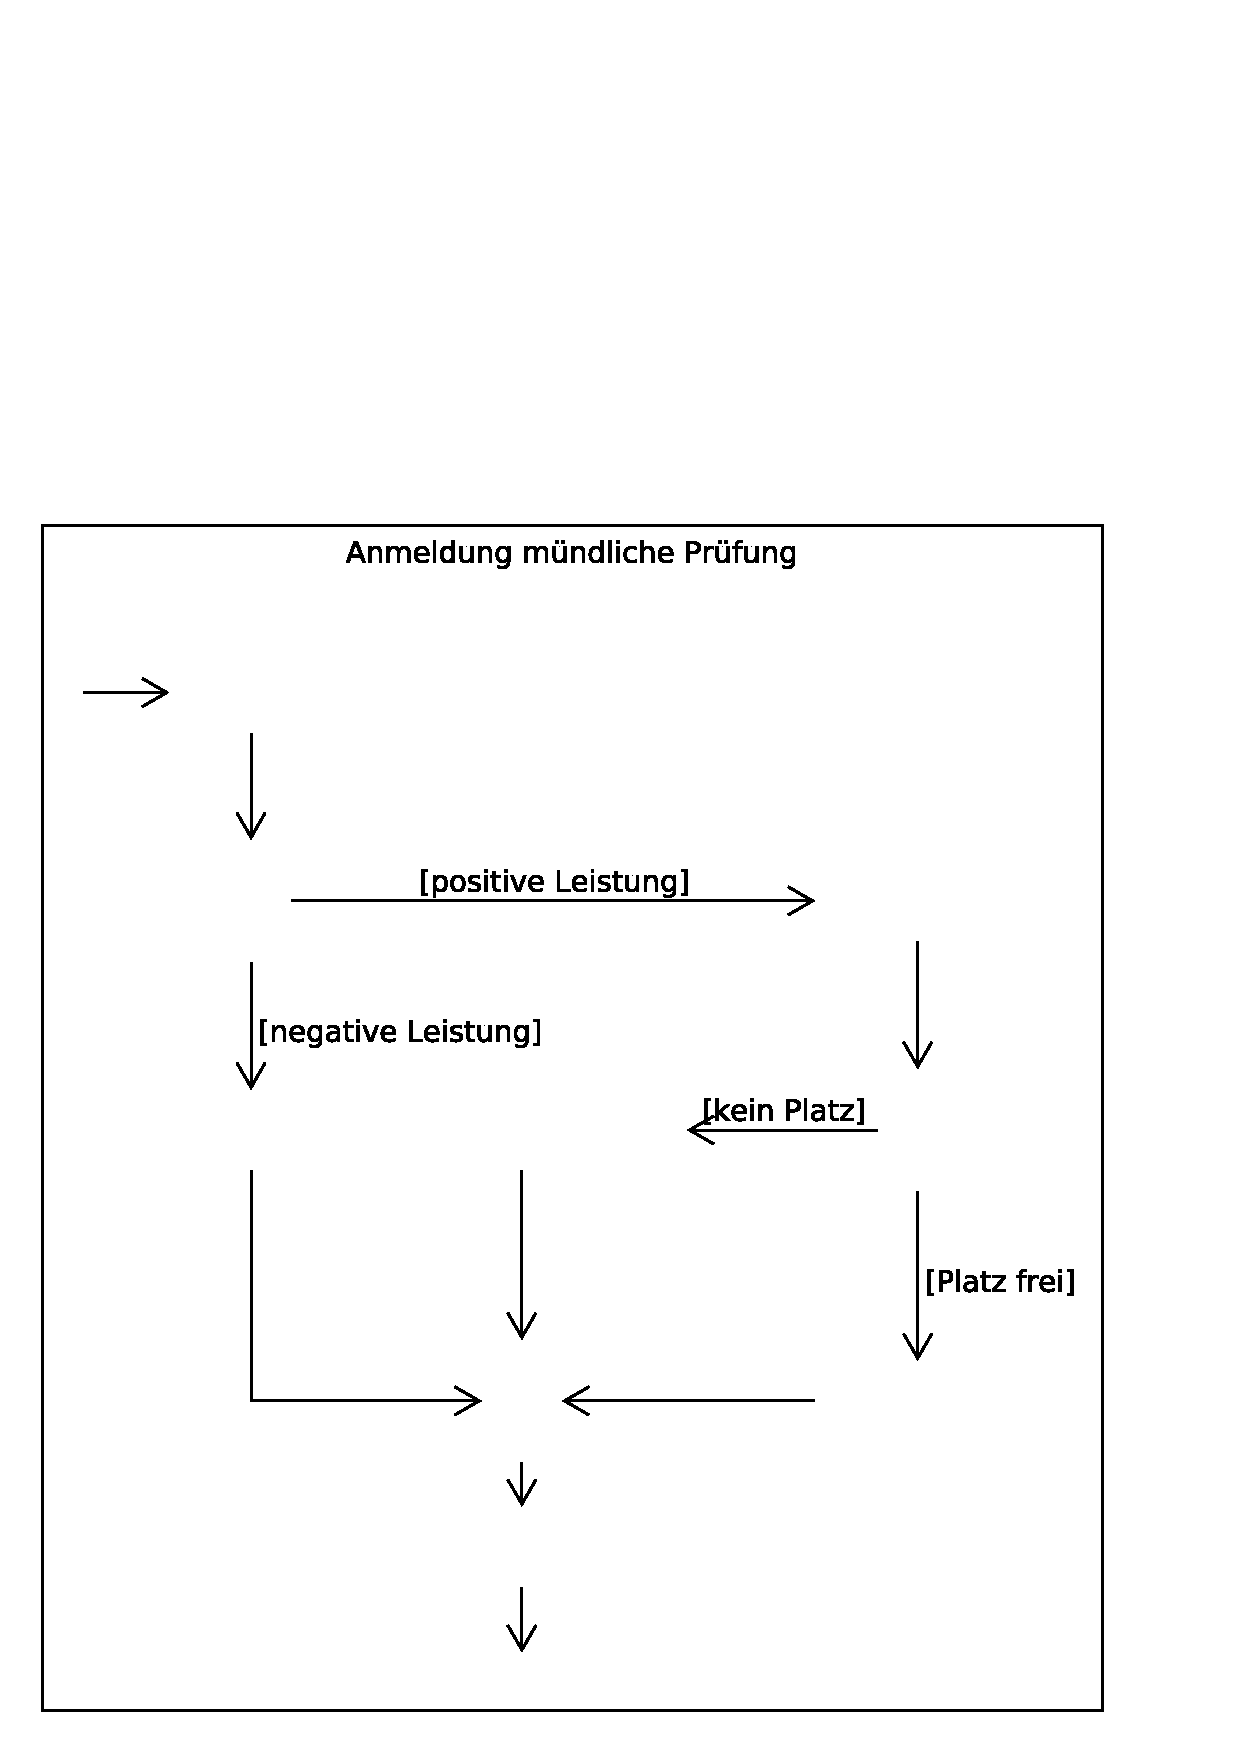
\includegraphics[scale=0.6]{Aufgabe1b.pdf}
        \end{center}

      \item Partitionen ermöglichen das Gruppieren von Knoten und Kanten nach
            bestimmten Kriterien. Damit kann man zB. zeigen, dass gewisse Aktionen
            Teil einer bestimmten Anwendung sind.
\newpage
      \item \hfill
        \begin{center}
           \includegraphics[scale=0.7]{Aufgabe1d.pdf}
         \end{center} 
    \end{enumerate}
  \end{solution}
  
  
  \problemnumber{2}
  \begin{problem}
    
  \end{problem}
  \begin{solution}\hfill
    \begin{enumerate}[label=\alph*)]\itemsep0pt
      \item Ein Token ist eine Art Marke, die auf den Kanten „wandert“. Tokens 
            werden verwendet um Abläufe zu koordinieren.

      \item Parallelisierungsknoten duplizieren alle eingehenden Tokens für alle
            ausgehenden Kanten. Der Synchronisierungsknoten ist das Gegenstück zum
            Parallelisierungsknoten und bewirkt, das alle eingehenden Tokens auf
            alle ausgehenden Kanten heruntergebrochen werden. \\
            Der Entscheidungsknoten stellt eine Weiche für die eingehenden Tokens.
            Je nach Antwort auf die Entscheidung wird der Ablauf fortgesetzt.
            Der Vereinigungsknoten ist das Gegenstück zum Entscheidungsknoten
            und ermöglicht es unterschiedliche Kanten zusammen zu führen. Hier 
            muss nur eine eingehende Kante mit einem Token belegt sein, damit 
            der Ablauf weitergeht.

      \item Die ersten beiden Konstrukte sind äquivalent, da der Startknoten jeder
            ausgehenden Kante ein Token zur Verfügung stellt. Der Parallelisierungsknoten
            tut dasselbe. \\
            Diese beiden sind nicht äquivalent, da im ersten Konstrukt sowohl Action2
            als auch Action3 ein Token erhalten, wobei das im zweiten Konstrukt
            nicht der Fall ist. \\
            Diese beiden Konstrukte sind nicht äquivalent, weil Action3 im ersten
            ausgeführt wird, wenn ein Token oder beide anliegen. Im Gegensatz
            zum zweiten Konstrukt, wo nur Action3 ausgeführt wird, wenn an allen
            eingehenden Kanten ein Token anliegt. \\
            Das erste und das dritte Konstrukt sind gleich, da auch an nur einer
            Kante ein Token sein kann. Das in der Mitte benötigt zwei Token, sodass
            an allen eingehenden Kanten ein Token anliegt.
    \end{enumerate}
    
  \end{solution}
  
  
  \problemnumber{3}
  \begin{problem}
    
  \end{problem}
  \begin{solution}\hfill
    \begin{enumerate}[label=\alph*)]\itemsep0pt
      \item Aktivitätsendknoten beenden alle Abläufe einer Aktivität wenn auch nur
            ein Token dorthin gelangt. Ablaufendknoten entfernen nur genau den Token,
            der gerade am Ablaufendknoten angekommen ist. 

      \item \hfill
        \begin{center}
          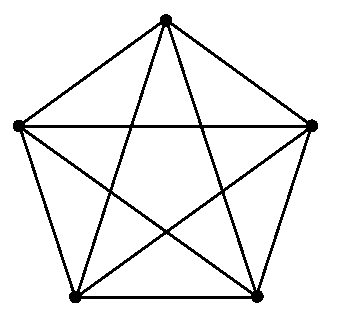
\includegraphics[scale=0.6]{Aufgabe3b.pdf}
        \end{center}

      \item \hfill
        \begin{center}
          \includegraphics[scale=0.55]{Aufgabe3c.pdf}
        \end{center}
    \end{enumerate}
  \end{solution}
  
  
  \problemnumber{4}
  \begin{problem}
    
  \end{problem}
  \begin{solution}
    
  \end{solution}
  
  
  \problemnumber{5}
  \begin{problem}
    
  \end{problem}
  \begin{solution}
    
  \end{solution}



\end{document}